\chapter{Results}
\label{cha:evaluation}

\section{Ester Formation}
Figure~\ref{fig:esters} shows the clear increase of isoamyl acetate with temperature.

\begin{figure}[htbp]
  \centering
  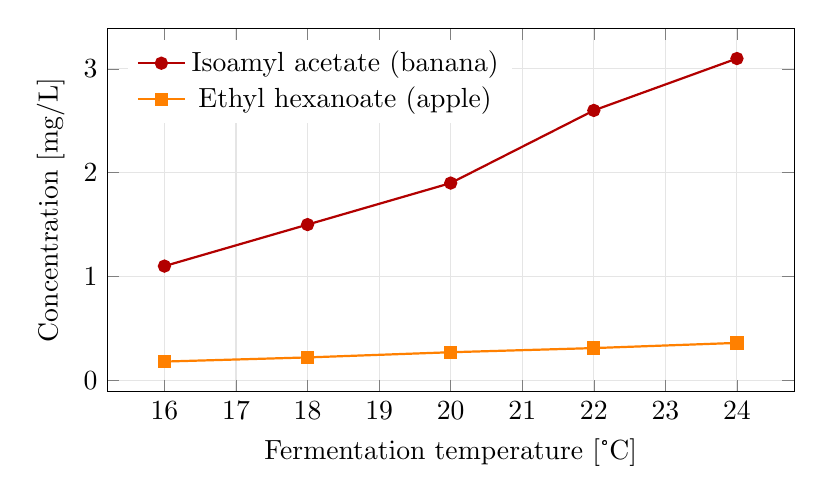
\begin{tikzpicture}
    \begin{axis}[
      width=0.85\linewidth, height=6.2cm,
      xlabel={Fermentation temperature [\textdegree{}C]}, ylabel={Concentration [mg/L]},
      grid=major, grid style={black!10},
      legend pos=north west, legend style={draw=none},
      every axis plot/.append style={thick}
    ]
      \addplot[color=red!70!black, mark=*] coordinates {(16,1.1) (18,1.5) (20,1.9) (22,2.6) (24,3.1)};
      \addplot[color=orange, mark=square*] coordinates {(16,0.18) (18,0.22) (20,0.27) (22,0.31) (24,0.36)};
      \legend{Isoamyl acetate (banana), Ethyl hexanoate (apple)}
    \end{axis}
  \end{tikzpicture}
  \caption{Ester concentration depending on fermentation temperature (means, $n=3$).}
  \label{fig:esters}
\end{figure}

\section{Tasting}
From 20\,\textdegree{}C on, 88\,\% of the participants noticed the difference. The beer
fermented at 18\,\textdegree{}C received the best overall impression -- fruity, but still clean.

\section{Discussion}
The results agree with the kinetic expectation from Equation~\ref{eq:arrhenius}.
